Nas estruturas reticuladas usuais, admite-se que o efeito das imperfeições locais esteja atendido se for respeitado o valor de \textbf{momento fletor mínimo}.

O momento fletor mínimo é dado pela seguinte equação:
\begin{equation}
	\label{equacao-momento-fletor-minimo}
	M_{1d,\;min}=N_d\cdot(1,5+0,03\cdot h)
\end{equation}

Onde $N_d$ é a força normal de cálculo e $h$ é a altura da seção transversal na direção considerada (em \textbf{centímetros}).

Essa equação tem como função aplicar uma \textbf{excentricidade mínima} a qualquer estrutura, de forma a atender as \textbf{imperfeições geométricas} executivas e a \textbf{incerteza} do \textbf{ponto exato} de aplicação das reações das vigas sobre os pilares.

Sendo assim, a excentricidade mínima é dada por:
\begin{equation}e_{1d,\;min}=1,5+0,03\cdot h\end{equation}

A Equação~\eqref{equacao-momento-fletor-minimo} também pode ser apresentada da seguinte forma:
\begin{equation}M_{1d,\;min}=N_d\cdot e_{1d,\;min}\end{equation}

\textbf{Exercício}: Calcular o momento fletor mínimo e as excentricidades nas duas direções e informar o tipo de pilar de acordo com seu Índice de Esbeltez, sabendo-se que: $N_k=785,7\;kN$, pilar (50x17) e $L_{ex}=L_{ey}=2,8\;m$.

\begin{figure}[H]
	\begin{center}
	\caption{Seção transversal de um pilar (50x17).}
    	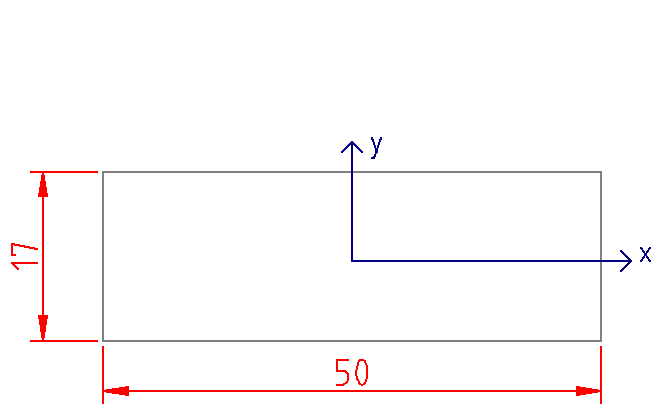
\includegraphics[width=0.4\textwidth]{Momento-fletor-minimo/Imagens/Secao-transversal-pilar-50x17.png}
	\end{center}
\end{figure}

Como $N_d$ depende da menor espessura do pilar, tem-se:
$$N_d=\gamma_f\cdot\gamma_n\cdot N_k=1,4\cdot1,1\cdot785,7\;kN=1209,9780\;kN$$

Para a direção $x$:
$$e_{1d,\;min\;x}=1,5+0,03\cdot h_x=1,5+0,03\cdot50=3\;cm$$
$$M_{1d,\;min\;x}=N_d\cdot e_{1d,\;min\;x}=1209,978\;kN\cdot3\;cm=3629,9340\;kN\cdot cm$$
$$\lambda_x=\frac{\sqrt{12}\cdot L_{ex}}{h_x}=\frac{\sqrt{12}\cdot2,8}{0,5}\approx19,3989$$

Para a direção $y$:
$$e_{1d,\;min\;y}=1,5+0,03\cdot h_y=1,5+0,03\cdot17=2,01\;cm$$
$$M_{1d,\;min\;y}=N_d\cdot e_{1d,\;min\;y}=1209,978\;kN\cdot2,01\;cm=2432,0557\;kN\cdot cm$$
$$\lambda_y=\frac{\sqrt{12}\cdot L_{ey}}{h_y}=\frac{\sqrt{12}\cdot2,8}{0,17}\approx57,0557$$

Portanto, na classificação de acordo com o Índice de Esbeltez, o pilar pertence ao pior caso das duas direções ($\lambda_y=57,0557$). É um pilar médio.